

\subsection{Stochastic Environment Model}\label{subsec:stochasticEnvModel}
Model-based agents require a concrete implementation of a model of their world, in order to maintain their internal state \cite[p~.50]{AIAMA}. The agent's internal state can be thought of as its opinion of what state the world might be in, and its model describes how it believes the world changes over time \cite{AIAMA}. Chapter \ref{chapter:Background} outlines the background behind potential models of the stochastic world, including both how internal state can be represented and how internal state can be updated.\par
Hidden Markov Models and Dynamic Bayesian Networks were identified as suitable models, due to the fact that they provide a succinct and flexible representation of hidden stochastic world state, as well as efficient online state estimation updating algorithms. We chose to use a Dynamic Bayesian Network (DBN), due to the fact that it can use conditional independence relations between variables to reduce the number of probabilities needed to be calculated to perform accurate inference \cite[p.~63]{KollerPGM}. DBNs also facilitate the incorporation of extra variables with arbitrary conditional independence relations. This was desirable, since we plan future work to extend the model to include extra variables, such as battery level, once a basic implementation was shown to work as intended.

The 2-Time Slice DBN shown in Figure \ref{fig:FirstDBNUsed} describes the agent's world model. A first-order Markov assumption is made, where the current state only depends on the state directly preceding it. Grey coloured variables are \textit{hidden state variables} and are assumed to not be directly observable. Green coloured variables are \textit{control actions} taken by the agent and the peach coloured variables are \textit{evidence variables}, which are assumed to be observable and depend on the hidden world state. 
%The agent's location and the search status hidden state variables are mainly included for technical reasons
\note{maybe re-position figure so text wraps}
\begin{figure}
    \centering
    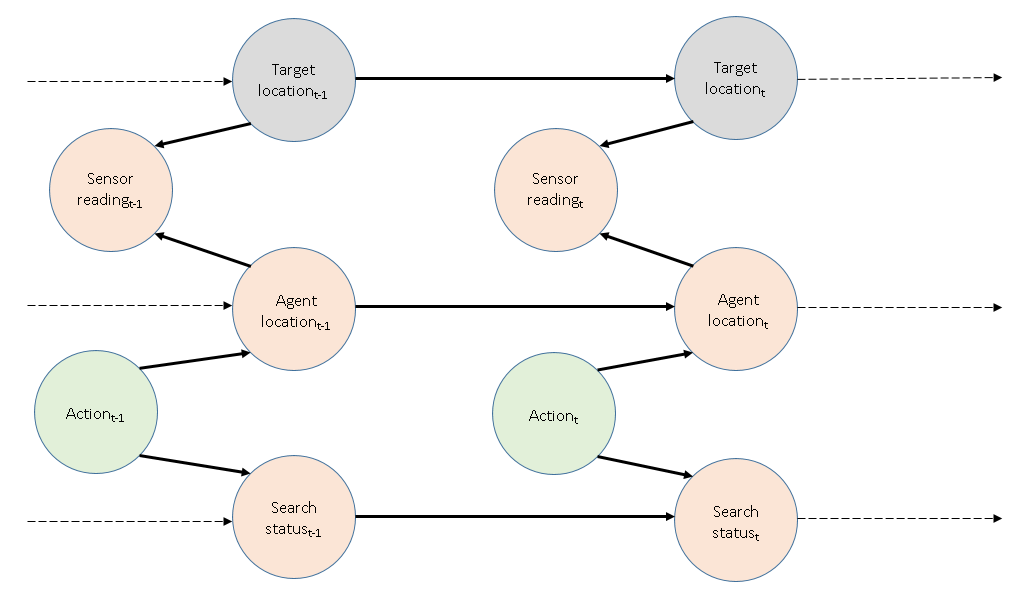
\includegraphics[width = 0.8\linewidth]{Chapters/MultiAgentTargetDetection/Figs/DBNs/DBNWithMultipleObservable.PNG}
     \caption{First Version of the DBN representing the agent world model}
    \label{fig:FirstDBNUsed}
\end{figure}
A number of conditional probabilities are specified here in order to describe the factored joint distribution of the world model fully. The full tables are omitted as they are sparse. For brevity, we use the abbreviation Loc for Location.



%\begin{figure}[H]
\scriptsize
\begin{equation}\label{eqn:EvidenceVarsProbs}
    %\centering
    p(SensorReading_t | AgentLoc_{t}, TargetLoc_{t})  = 
    \begin{cases}
    \alpha \quad \text{ if } SensorReading_t=1 \text{ and } TargetLoc_t \neq AgentLoc_t
    \\
    1-\beta \quad \text{ if } SensorReading_t=1 \text{ and } TargetLoc_t = AgentLoc_t
    \\
    \beta \quad \text{ if } SensorReading_t=0 \text{ and } TargetLoc_t = AgentLoc_t
    \\
    1-\alpha \quad \text{ if } SensorReading_t=0 \text{ and } TargetLoc_t \neq AgentLoc_t
    \end{cases}
    %
\end{equation}
\begin{center}
    \normalsize
    Conditional Probability Distribution for the $Evidence$ Variable.
\end{center}
%\caption{Conditional Probability Distribution for the $Evidence$ Variable}
%\end{figure}


%\begin{figure}[H]
\scriptsize
\begin{equation}\label{eqn:TargetLocProbs}
    p(TargetLoc_{t} | TargetLoc_{t-1}) =
    \begin{cases}
    1 \quad \text{ if } TargetLoc_{t}=TargetLoc_{t-1}
    %agent returns correct target Loc.} 
    \\
    0 \quad \text { otherwise. }
    \end{cases}
\end{equation}
%\caption{Conditional Probability Distribution for the $TargetLocation$ Variable}
%\end{figure}
\begin{center}
\normalsize
    Conditional Probability Distribution for the $TargetLocation$ Variable
\end{center}





%\begin{figure}[H]
\scriptsize
%\begin{equation}\label{eqn:SearchStatus}
    \begin{gather}\label{eqn:SearchStatus}
        p(SearchStatus_t | SearchStatus_{t-1}, Action_{t-1}) = \\
        \begin{cases}
        1 \quad \text{ if } SearchStatus_t = terminated\_x_i \text{ and } SearchStatus_{t-1} = terminated\_x_i 
        \\
        1 \quad \text{ if } Action_t = terminate\_x_i \text{ and } SearchStatus_{t-1}=ongoing \text{ and } SearchStatus_{t} = terminated\_x_i
        \\
        1 \quad \text{ if } Action_t = move\_x_i \text{ and } SearchStatus_{t-1}=ongoing \text{ and } SearchStatus_t=ongoing
        %agent returns correct target location.} 
        \\
        0 \quad \text { otherwise. }
        \end{cases}
    \end{gather}
%\end{equation}
%\caption{Conditional Probability Distribution for the $SearchStatus$ Variable}
%\end{figure}
\begin{center}
    \normalsize
    Conditional Probability Distribution for the $SearchStatus$ Variable
\end{center}




%\begin{figure}[H]
\scriptsize
    \begin{equation}\label{eqn:AgentLocation}
        p(AgentLoc_t | AgentLoc_{t-1}, Action_{t}) = 
        \begin{cases}
        1 \quad \text{ if } Action_t = move\_x_i \text{ and } AgentLoc_t = x_i
        \\
        1 \quad \text{ if } Action_t = terminate\_x_i \text{ and } AgentLoc_t = AgentLoc_{t-1}
        \\
        0 \quad \text{otherwise}
        \end{cases}
    \end{equation}
%\caption{Conditional Probability Distribution for the $AgentLocation$ Variable}
%\end{figure}
\begin{center}
    \normalsize
    Conditional Probability Distribution for the $AgentLocation$ Variable
\end{center}

\normalsize
The semantics of the equations listed above is given here: 
\begin{enumerate}
    \item Equation \ref{eqn:EvidenceVarsProbs} uses two parameters, $\alpha$ and $\beta$, to represent the probability of making a false positive and false negative sensor reading, respectively. These are assumed to have been calculated by using pre-calibrated values of the sensor. This model is does not stipulate any restrictions on the sensor other than that it must return a reading indicating that the target is present or not.
    \item  Equation \ref{eqn:TargetLocProbs} simply states that the location of the target does not change, even though it is hidden. This could be modified to allow for mobile target detection in the case of a non-stationary target by introducing non-unity probabilities in a transition matrix for different values of $TargetLoc_t$ and $TargetLoc_{t-1}$.
    \item The first line of Equation \ref{eqn:SearchStatus} states that once the agent terminates the search, it remains over. The second line states that if the agent requests an ongoing search to terminate, then it does so deterministically. The third line states that if the agent chooses to move in an ongoing search, then the search remains ongoing.
    \item Equation \ref{eqn:AgentLocation} states that the agent moves to new locations deteministically. It also indicates that should the agent choose to terminate the search, then the environment enters a terminal state, indicating that the search is over.
\end{enumerate}


Note that despite the fact that some hidden state variables cannot be observed directly, it is still possible to infer their value exactly based on their starting state. For example, the position of the agent is a deterministic function of its actions and previous position. %These variables could have been treated as variables that are internal to the agent rather than part of the hidden world state and could have been omitted for the sake of clarity.
%many authors 
%\note{need to outline why I have included them - mainly because evidence probability depends on agent location as well as source location}


%\subsection{Analysis of Stochastic Environment Model}
%\note{talk about evolution of belief given a sequence of null observations}